\documentclass[11pt]{article}
\usepackage[utf8]{inputenc}
\usepackage[T1]{fontenc}
\usepackage{amsmath}
\usepackage{amssymb} % Needed for \eth
\usepackage{graphicx}
\usepackage{geometry}
\usepackage{tikz}
\usepackage{pgfplots} % For plots
\usepackage{ulem}     % For underline, using normalem to avoid messing with \emph
\usepackage{tcolorbox} % For boxing equations if needed
\usepackage{braket}    % For QM state notation if needed

\geometry{a4paper, margin=1in}
\usetikzlibrary{positioning, arrows.meta, shapes.geometric, patterns, calc} % Added calc library
\pgfplotsset{compat=1.18} % Use a recent PGFPlots version

% Custom commands (optional)
\newcommand{\avg}[1]{\overline{#1}}
\newcommand{\prob}[1]{P(#1)}
\newcommand{\ProbDens}[1]{\mathcal{P}(#1)} % Using script P for density
\newcommand{\vect}[1]{\vec{#1}}
\newcommand{\dd}[1]{\mathrm{d}#1} % Differential d
\newcommand{\pderiv}[2]{\frac{\partial #1}{\partial #2}}
\newcommand{\deriv}[2]{\frac{\mathrm{d} #1}{\mathrm{d} #2}}
\newcommand{\muState}{\mu\text{-state}} % Microstate
\newcommand{\OmegaE}{\Omega(E)}
\newcommand{\omegaE}{\omega(E)}
\newcommand{\PhiE}{\Phi(E)}
\newcommand{\deltaE}{\delta E}
\newcommand{\ethbar}{\text{\it{đ}}} % \eth symbol for inexact differential
\newcommand{\kb}{k_B} % Boltzmann constant (set to 1 unless specified)
\newcommand{\gasR}{R} % Ideal gas constant
\newcommand{\partfn}{Z} % Partition function symbol
\newcommand{\grandpartfn}{\mathcal{Z}} % Grand partition function symbol
\newcommand{\lambdaT}{\lambda_{th}} % Thermal wavelength
\newcommand{\eps}{\epsilon}
\newcommand{\nbar}{\overline{n}} % Mean occupation number

\title{Physics 415 - Lecture 36: Black-Body Radiation Thermodynamics}
\date{April 21, 2025}
\author{} % Author not specified

\begin{document}

\maketitle
\thispagestyle{empty}

\section*{Summary}

\begin{itemize}
    \item Black-body radiation = equilibrium EM radiation $\approx$ photon gas.
    \item Single-particle photon state specified by $(\vec{k}, \alpha)$, where $\vec{k}$ is wave-vector and $\alpha=1, 2$ is polarization $\perp \vec{k}$.
    \item Energy $\eps_k = \hbar ck = \hbar\omega$.
    \item Mean occupation number (Planck distribution): $\nbar_{k\alpha} = \frac{1}{e^{\beta\hbar\omega}-1}$ (since $\mu=0$).
    \item Counting states: $\sum_r \to \sum_{\vec{k},\alpha} \to 2 V \int \frac{d^3k}{(2\pi)^3} \to \int_0^\infty d\omega \, g(\omega)$, where $g(\omega) = \frac{V\omega^2}{\pi^2 c^3}$ is density of modes per frequency.
    \item Spectral energy density (Planck's formula): $u(\omega) = \frac{1}{V}\frac{dE}{d\omega} = g(\omega)/V \times \nbar(\omega) \times \hbar\omega = \frac{\hbar}{\pi^2 c^3} \frac{\omega^3}{e^{\beta\hbar\omega}-1}$.
    \item Total energy density (Stefan-Boltzmann Law): $u = \frac{E}{V} = \int_0^\infty u(\omega) d\omega = \frac{\pi^2 T^4}{15 (\hbar c)^3}$. ($T$ in energy units, $k_B=1$).
\end{itemize}

\section*{Thermodynamic Quantities for Black-Body Radiation}

\subsection*{Free Energy (F)}
Photons obey photon statistics (BE with $\mu=0$). The Helmholtz free energy is $F = T \sum_r \ln(1 - e^{-\beta\eps_r})$.
Convert sum to integral:
\[ F = T \sum_{\alpha=1,2} V \int \frac{d^3k}{(2\pi)^3} \ln(1 - e^{-\beta\hbar ck}) \]
\[ F = 2 T V \int_0^\infty \frac{4\pi k^2 dk}{(2\pi)^3} \ln(1 - e^{-\beta\hbar ck}) \]
\[ F = \frac{T V}{\pi^2} \int_0^\infty k^2 dk \ln(1 - e^{-\beta\hbar ck}) \]
Change variable to frequency $\omega=ck$, $k=\omega/c$, $dk=d\omega/c$:
\[ F = \frac{T V}{\pi^2 c^3} \int_0^\infty \omega^2 d\omega \ln(1 - e^{-\beta\hbar\omega}) \]
Change variable to dimensionless $x = \beta\hbar\omega = \hbar\omega/T$. $\omega = Tx/\hbar$, $d\omega = Tdx/\hbar$.
\[ F = \frac{T V}{\pi^2 c^3} \int_0^\infty \left(\frac{Tx}{\hbar}\right)^2 \left(\frac{Tdx}{\hbar}\right) \ln(1 - e^{-x}) \]
\[ F = \frac{V T^4}{\pi^2 (\hbar c)^3} \int_0^\infty dx \, x^2 \ln(1 - e^{-x}) \]
Integrate by parts: $u = \ln(1-e^{-x})$, $dv = x^2 dx \implies v = x^3/3$.
$\int_0^\infty u dv = [uv]_0^\infty - \int_0^\infty v du$.
$du = \frac{-(-e^{-x})}{1-e^{-x}} dx = \frac{e^{-x}}{1-e^{-x}} dx = \frac{1}{e^x-1} dx$.
\[ \int_0^\infty x^2 \ln(1-e^{-x}) dx = \left[ \frac{x^3}{3} \ln(1-e^{-x}) \right]_0^\infty - \int_0^\infty \frac{x^3}{3} \frac{1}{e^x-1} dx \]
The boundary term is zero at $x=0$ (since $x^3=0$) and at $x=\infty$ (since $\ln(1)=0$).
The remaining integral is $\int_0^\infty \frac{x^3}{e^x-1} dx = \frac{\pi^4}{15}$.
So, $\int_0^\infty x^2 \ln(1-e^{-x}) dx = -\frac{1}{3} \frac{\pi^4}{15} = -\frac{\pi^4}{45}$.
Substitute back into $F$:
\[ F = \frac{V T^4}{\pi^2 (\hbar c)^3} \left( -\frac{\pi^4}{45} \right) = - V \frac{\pi^2 T^4}{45 (\hbar c)^3} \]

\subsection*{Check Energy and Pressure}
\begin{itemize}
    \item Energy $E$: Use $E = F+TS$. First find $S = -(\partial F/\partial T)_V$.
    \[ S = -\pderiv{}{T} \left( - V \frac{\pi^2 T^4}{45 (\hbar c)^3} \right)_V = V \frac{\pi^2}{45 (\hbar c)^3} (4T^3) \]
    \[ E = F + TS = - V \frac{\pi^2 T^4}{45 (\hbar c)^3} + T \left( V \frac{4\pi^2 T^3}{45 (\hbar c)^3} \right) \]
    \[ E = V \frac{\pi^2 T^4}{(\hbar c)^3} \left( -\frac{1}{45} + \frac{4}{45} \right) = V \frac{\pi^2 T^4}{(\hbar c)^3} \frac{3}{45} = V \frac{\pi^2 T^4}{15 (\hbar c)^3} \]
    This matches the Stefan-Boltzmann law $u = E/V = \frac{\pi^2 T^4}{15 (\hbar c)^3}$. $\checkmark$
    \item Pressure $p$: Use $p = -(\partial F/\partial V)_T$.
    \[ p = -\pderiv{}{V} \left( - V \frac{\pi^2 T^4}{45 (\hbar c)^3} \right)_T = \frac{\pi^2 T^4}{45 (\hbar c)^3} \]
    Note the relation between pressure and energy density $u=E/V$:
    \[ p = \frac{1}{3} \left( \frac{\pi^2 T^4}{15 (\hbar c)^3} \right) = \frac{1}{3} u \]
    So, $pV = \frac{1}{3} E$. This is the equation of state for a photon gas ("radiation pressure").
    (Compare with $pV = \frac{2}{3} E$ for non-relativistic ideal gas).
\end{itemize}

\subsection*{Total Number of Photons}
The total number of photons $N$ is not fixed, but we can calculate its average value.
\[ N = \avg{N} = \sum_r \nbar_r = \int_0^\infty d\omega \, g(\omega) \nbar(\omega) \]
\[ N = \int_0^\infty d\omega \left( \frac{V \omega^2}{\pi^2 c^3} \right) \frac{1}{e^{\beta\hbar\omega} - 1} \]
Let $x=\beta\hbar\omega$. $\omega = Tx/\hbar$, $d\omega=Tdx/\hbar$.
\[ N = \frac{V}{\pi^2 c^3} \int_0^\infty \left(\frac{Tx}{\hbar}\right)^2 \frac{1}{e^x - 1} \left(\frac{Tdx}{\hbar}\right) = \frac{V T^3}{\pi^2 (\hbar c)^3} \int_0^\infty dx \frac{x^2}{e^x - 1} \]
The integral is $\int_0^\infty \frac{x^{s-1}}{e^x-1} dx = \Gamma(s)\zeta(s)$. Here $s-1=2 \implies s=3$.
Integral $= \Gamma(3)\zeta(3) = 2! \zeta(3) = 2 \zeta(3)$, where $\zeta(3) \approx 1.202$.
\[ N = \frac{V T^3}{\pi^2 (\hbar c)^3} (2\zeta(3)) \]
The number density of photons is $n = N/V$:
\[ n = \frac{2 \zeta(3)}{\pi^2} \left( \frac{T}{\hbar c} \right)^3 \approx 0.244 \left( \frac{T}{\hbar c} \right)^3 \]
In equilibrium, the density of photons is determined solely by the temperature $T$.

\section*{Radiation Emitted by a Body at Temperature T}

So far, considered equilibrium radiation *inside* an enclosure at temperature $T$. Now consider the radiation *emitted* by a body whose surface is at temperature $T$.
A body in thermal equilibrium with black-body radiation continually reflects \& absorbs incident photons, and also emits new photons. In equilibrium, these processes balance, and the photon distribution $\nbar_{k\alpha}$ remains unchanged.

\begin{center}
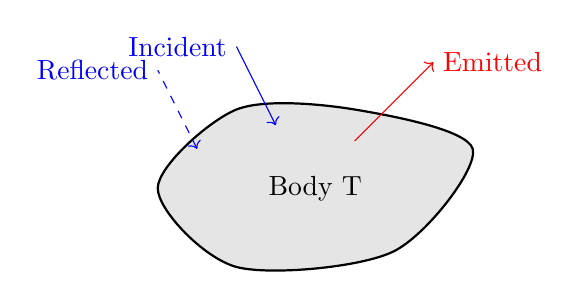
\begin{tikzpicture}
    % Body surface
    \draw [thick, fill=gray!20] plot [smooth cycle] coordinates {(-2,0) (-1, -1) (1,-0.8) (2,0.5) (0.5,1) (-1,1)};
    \node at (0,0) {Body T};
    % Incident radiation
    \draw [->, blue] (-1, 1.8) node[left]{Incident} -- (-0.5, 0.8);
    % Reflected radiation
    \draw [<-, blue, dashed] (-1.5, 0.5) -- (-2, 1.5) node[left] {Reflected};
    % Absorbed (implicit)
    % Emitted radiation
    \draw [->, red] (0.5, 0.6) -- (1.5, 1.6) node[right] {Emitted};
\end{tikzpicture}
\end{center}
Question: How much power does the body emit by radiation as a function of frequency $\omega$?

Let $J(\omega, \theta) d\omega d\Omega$ = Power emitted per unit area of the body surface into a small solid angle $d\Omega$ around direction $\hat{k}$, within frequency range $(\omega, \omega+d\omega)$. The angle $\theta$ is between $\hat{k}$ and the surface normal $\hat{n}$ ($\cos\theta = \hat{k}\cdot\hat{n}$). Summed over polarization.

\begin{center}
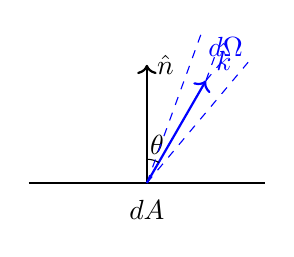
\begin{tikzpicture}
    % Surface element
    \draw [fill=gray!20] (-1.5,0) -- (1.5,0); \node at (0,-0.1) [below] {$dA$};
    \draw [thick] (-1.5,0) -- (1.5,0);
    % Normal
    \draw [->, thick] (0,0) -- (0,1.5) node[right] {$\hat{n}$};
    % Direction k
    \coordinate (O) at (0,0);
    \coordinate (K) at (60:1.5); % Angle theta = 30 deg
    \draw [->, blue, thick] (O) -- (K) node[above right] {$\hat{k}$};
    % Angle theta
    \draw (0,0.3) arc (90:60:0.3); \node at (75:0.5) {$\theta$};
    % Solid angle dOmega
    \draw [dashed, blue] (K) -- ++(50:0.4); \draw [dashed, blue] (K) -- ++(70:0.4);
    \draw [dashed, blue] (O) -- ++(50:2); \draw [dashed, blue] (O) -- ++(70:2);
    \node at (60:2) [blue] {$d\Omega$};
\end{tikzpicture}
\end{center}

First consider radiation incident on the body from the equilibrium field at temperature $T$.
Energy density of photons in $(\omega, \omega+d\omega)$ is $u_\omega d\omega = \frac{\hbar}{\pi^2 c^3} \frac{\omega^3 d\omega}{e^{\beta\hbar\omega}-1}$.
Energy incident on $dA$ from $d\Omega$ about $\hat{k}$ in time $dt$:
$dE_{inc} = (u_\omega d\omega) \times (\frac{d\Omega}{4\pi}) \times (c dt \cos\theta dA)$.
($\frac{d\Omega}{4\pi}$ = fraction of isotropic photons in $d\Omega$. $c dt \cos\theta dA$ = volume containing photons hitting $dA$).
Incident power per unit area from $d\Omega, d\omega$:
\[ \frac{dP_{inc}}{dA} = \frac{dE_{inc}}{dA dt} = \frac{c u_\omega \cos\theta}{4\pi} d\omega d\Omega \]
\[ \frac{dP_{inc}}{dA} = \frac{\hbar \omega^3}{4\pi^3 c^2} \frac{\cos\theta}{e^{\beta\hbar\omega}-1} d\omega d\Omega \]
In general, only a fraction $a(\omega, \theta)$ (absorptivity) of incident radiation is absorbed, the rest is reflected.
Power absorbed per unit area from $d\Omega, d\omega$:
\[ \frac{dP_{abs}}{dA} = a(\omega, \theta) \frac{dP_{inc}}{dA} = a(\omega, \theta) \frac{c u_\omega \cos\theta}{4\pi} d\omega d\Omega \]
In equilibrium, the energy of the body is unchanged, so radiated power must balance absorbed power for each $(\omega, \theta, d\Omega, d\omega)$:
\[ J(\omega, \theta) d\omega d\Omega = \frac{dP_{abs}}{dA} = a(\omega, \theta) \frac{c u_\omega \cos\theta}{4\pi} d\omega d\Omega \]
\[ \implies J(\omega, \theta) = a(\omega, \theta) \frac{c u_\omega \cos\theta}{4\pi} \]
The functions $J(\omega, \theta)$ (emissivity) and $a(\omega, \theta)$ (absorptivity) are determined solely by properties of the body at temperature $T$. But their ratio is a universal function of $\omega, T, \theta$, independent of the body:
\[ \frac{J(\omega, \theta)}{a(\omega, \theta)} = \frac{c u_\omega \cos\theta}{4\pi} = \frac{\hbar \omega^3}{4\pi^3 c^2} \frac{\cos\theta}{e^{\beta\hbar\omega}-1} \]
This is \textbf{Kirchhoff's Law}: A good emitter of radiation is also a good absorber (and vice-versa).

\subsection*{Black Body Emission}
Important special case: $a(\omega, \theta) = 1$ for all $\omega, \theta$. The body absorbs all incident radiation. Such a body is called a "black body" (at $T=0$ K, it would look black).
For a black body:
\[ J_{bb}(\omega, \theta) = \frac{c u_\omega \cos\theta}{4\pi} = \frac{\hbar \omega^3}{4\pi^3 c^2} \frac{\cos\theta}{e^{\beta\hbar\omega}-1} \]
The emitted power is entirely determined by the equilibrium radiation field at temperature $T$. In particular, the emitted power is the same for all black bodies at the same $T$.

\textbf{Model of a Black Body:} A cavity with highly absorbing walls and a small hole.

\begin{center}
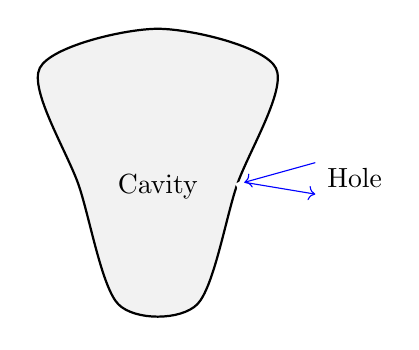
\begin{tikzpicture}
    % Cavity shape
    \draw [thick, fill=gray!10] plot [smooth cycle] coordinates {(-1,0) (-1.5,1.5) (0,2) (1.5,1.5) (1,0) (0.5, -1.5) (-0.5, -1.5)};
    % Hole
    \draw [line width=2pt, white] (1,0) -- (1.2, 0.1); % Erase part of boundary
    \node at (0,0) {Cavity};
    % Incident/Outgoing rays
    \draw [->, blue] (2, 0.3) -- (1.1, 0.05);
    \draw [<-, blue] (2, -0.1) -- (1.1, 0.05);
    \node at (2.5, 0.1) {Hole};
\end{tikzpicture}
\end{center}
Any radiation incident on the hole enters the cavity and has negligible probability of escaping after repeated reflections from the (absorbing) cavity walls. The hole effectively absorbs all incident radiation and acts as a black body surface. The radiation emerging from the hole is characteristic of the equilibrium radiation inside at temperature $T$.

\subsection*{Total Radiated Power}

Compute the total power per unit area radiated by a black body in frequency range $(\omega, \omega+d\omega)$, denoted $J_\omega d\omega$. Integrate $J_{bb}(\omega, \theta)$ over the outgoing hemisphere ($d\Omega = \sin\theta d\theta d\phi$, $\theta \in [0, \pi/2]$).
\[ J_\omega d\omega = \left( \int_{\text{hemisphere}} J_{bb}(\omega, \theta) d\Omega \right) d\omega \]
\[ J_\omega d\omega = \left( \int_0^{2\pi} d\phi \int_0^{\pi/2} d\theta \sin\theta \, a(\omega,\theta) \frac{c u_\omega \cos\theta}{4\pi} \right) d\omega \]
Assuming $a=1$ for black body:
\[ J_\omega = \frac{c u_\omega}{4\pi} \int_0^{2\pi} d\phi \int_0^{\pi/2} d\theta \sin\theta \cos\theta \]
The angular integral is $(2\pi) \times [\frac{1}{2}\sin^2\theta]_0^{\pi/2} = (2\pi)(1/2) = \pi$.
\[ J_\omega = \frac{c u_\omega}{4\pi} (\pi) = \frac{c}{4} u_\omega \]
\[ J_\omega = \frac{c}{4} \frac{\hbar}{\pi^2 c^3} \frac{\omega^3}{e^{\beta\hbar\omega}-1} = \frac{\hbar}{4\pi^2 c^2} \frac{\omega^3}{e^{\beta\hbar\omega}-1} \]
This is the Planck law for the spectral distribution of power emitted by a black body.

Total power per unit area radiated over all frequencies, $J$:
\[ J = \int_0^\infty J_\omega d\omega = \int_0^\infty \frac{c}{4} u_\omega d\omega = \frac{c}{4} \int_0^\infty u_\omega d\omega \]
The integral is the total energy density $u = \frac{\pi^2 T^4}{15 (\hbar c)^3}$.
\[ J = \frac{c}{4} \left( \frac{\pi^2 T^4}{15 (\hbar c)^3} \right) = \frac{\pi^2 T^4}{60 \hbar^3 c^2} \]
If $T$ is in Kelvin, use $T_{energy} = \kb T_{Kelvin}$:
\[ J = \frac{\pi^2 (\kb T)^4}{60 \hbar^3 c^2} = \left( \frac{\pi^2 \kb^4}{60 \hbar^3 c^2} \right) T^4 \]
\[ J = \sigma T^4 \]
This is the \textbf{Stefan-Boltzmann Law} for black-body emission.
The Stefan-Boltzmann constant is $\sigma = \frac{\pi^2 \kb^4}{60 \hbar^3 c^2}$.

\end{document}